\subsection{High availability and redundancy}

Some DCSs may require a 24/7 period availability, which means communication stability is crucial.
The most common network failures are a cable break or an intermediate node failure, both of which can prevent communication with downstream stations.
ESCs are prepared to adapt quickly in case of network failures, with link detection times below 15$\mu$s, losing at most one communication cycle.
So, if an additional cable is employed to connect the last slave device back to the master node, creating a ring topology (see \autoref{fig:ecat-redundancy}), access to all devices is guaranteed in the event of a cable breakage or device malfunction.

\begin{figure}[htp]
	\centering
	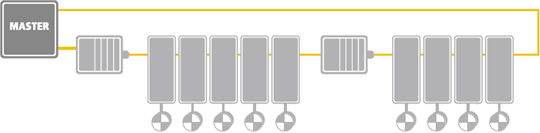
\includegraphics[width=0.8\textwidth]{EtherCAT_Technology_07_CableRedundancy.jpg}
	\caption{EtherCAT cable redundancy \cite{protocol:ethercat}}
	\label{fig:ecat-redundancy}
\end{figure}


